%%%%%%%%%%%%%%%%%%%%%%% file template.tex %%%%%%%%%%%%%%%%%%%%%%%%%
%
% This is a general template file for the LaTeX package SVJour3
% for Springer journals.          Springer Heidelberg 2010/09/16
%
% Copy it to a new file with a new name and use it as the basis
% for your article. Delete % signs as needed.
%
% This template includes a few options for different layouts and
% content for various journals. Please consult a previous issue of
% your journal as needed.
%
%%%%%%%%%%%%%%%%%%%%%%%%%%%%%%%%%%%%%%%%%%%%%%%%%%%%%%%%%%%%%%%%%%%
%
% First comes an example EPS file -- just ignore it and
% proceed on the \documentclass line
% your LaTeX will extract the file if required
% \begin{filecontents*}{example.eps}
%!PS-Adobe-3.0 EPSF-3.0
%%BoundingBox: 19 19 221 221
%%CreationDate: Mon Sep 29 1997
%%Creator: programmed by hand (JK)
%%EndComments
% gsave
% newpath
%   20 20 moveto
%   20 220 lineto
%   220 220 lineto
%   220 20 lineto
% closepath
% 2 setlinewidth
% gsave
%   .4 setgray fill
% grestore
% stroke
% grestore
% \end{filecontents*}
%
\RequirePackage{fix-cm}

%
%\documentclass{svjour3}                     % onecolumn (standard format)
%\documentclass[smallcondensed]{svjour3}     % onecolumn (ditto)
\documentclass[smallextended]{svjour3}       % onecolumn (second format)
%\documentclass[twocolumn]{svjour3}          % twocolumn
%
\smartqed  % flush right qed marks, e.g. at end of proof
%
\usepackage{graphicx}
%
% \usepackage{mathptmx}      % use Times fonts if available on your TeX system
%
% insert here the call for the packages your document requires
\usepackage[authoryear]{natbib}
\usepackage{siunitx}
\usepackage[hidelinks]{hyperref}
\usepackage{lineno}
\usepackage{setspace}
\usepackage{booktabs}
% \usepackage[utf8]{inputenc}
\doublespacing
%\usepackage{latexsym}
% etc.
%
% please place your own definitions here and don't use \def but
% \newcommand{}{}
%
% Insert the name of "your journal" with
\journalname{Estuaries and Coasts}
%
\begin{document}
\linenumbers

\title{Fine-scale relationships between phytoplankton abundance and environmental drivers in Florida Bay, USA%\thanks{Grants or other notes
%about the article that should go on the front page should be
%placed here. General acknowledgments should be placed at the end of the article.}
}
% \subtitle{Do you have a subtitle?\\ If so, write it here}

\titlerunning{Fine-scale phytoplankton abundance in Florida Bay}        % if too long for running head

\author{Joseph Stachelek         \and
        Christopher Madden  \and
        Stephen Kelly \and
        Michelle Blaha
}

%\authorrunning{Short form of author list} % if too long for running head

\institute{J. Stachelek \at
              South Florida Water Management District \\
              Everglades Systems Assessment Section \\
              West Palm Beach, FL 33406, USA \\
              \email{stachel2@msu.edu}             \\
              \emph{Present address:} of J. Stachelek  %  if needed
            \at
              Michigan State University \\
              East Lansing, MI, 48824, USA
}

\date{Edited: 2017-02-27 / Received: date / Accepted: date}
% The correct dates will be entered by the editor


\maketitle

\begin{abstract}
Phytoplankton abundance plays a critical role in structuring ecosystem processes in subtropical estuaries. The numerous factors that control phytoplankton abundance can be classified according to the spatial scale at which they operate. To date, most studies have focused either on micro-scale processes that control phytoplankton abundance such as nutrient availability or the influence of larger-scale regional processes such as climatic variability and global teleconnections. Inferences from these studies are often dependent on spatially-coarse discrete grab sampling networks whose spatial representativeness is unknown. In this study, we show that a combination of discrete sampling and underway flow-through sampling can provide important insights into the drivers of phytoplankton abundance as well as resolve the locations, shapes, and boundaries of water quality features in a quantitative and spatially explicit manner. In particular, we show the correspondence between elevated phytoplankton abundance and a number of parameters including phytopigment fluorescence and colored dissolved organic matter (CDOM) fluorescence in Florida Bay, USA.
\keywords{Everglades \and restoration \and water quality}
% \PACS{PACS code1 \and PACS code2 \and more}
% \subclass{MSC code1 \and MSC code2 \and more}
\end{abstract}

\section{Introduction}
\label{intro}
Phytoplankton abundance plays a critical role in structuring ecosystem processes in subtropical estuaries. For example, unusually high abundance reflects the onset of phytoplankton blooms which can decrease light penetration in the water column causing decreased seagrass growth and benthic productivity \citep{kelble_2005}. Furthermore, phytoplankton abundance is often used as an indirect measure of nutrient loading, eutrophication, and overall ecosystem status \citep{boyer_2009}. As such, it is important to understand the numerous factors that control phytoplankton abundance. One way to conceptualize these regulating factors is to organize them according to the spatial scale at which they operate. At a micro-scale ($<$ 1 m), abundance is regulated by nutrient availability, turbulence, and predation \citep{mann2013dynamics}. At larger spatial scales, abundance is regulated by a suite of processes including advective transport \citep{dugdale2012river}, benthic-pelagic coupling \citep{zhang_2014, lawrence2004wind} regional climate variability, and global teleconnections \citep{briceno_climatic_2009}.

Different approaches are necessary in order to investigate the regulation of phytoplankton dynamics by environmental factors at each of these scales. For example, information on micro-scale dynamics often comes from laboratory culture studies while information on larger scale dynamics comes from studies utilizing distributed grab sample networks. Some of these larger-scale studies are the result of long-term water quality monitoring efforts that have provided great insight into the seasonality and interannual variability associated with phytoplankton abundance across broad ($>10$ km) geographic scales \citep{cloern_patterns_2010}.

Although, distributed grab sampling networks are very effective at revealing trends over time, they are less effective at providing spatially explicit information at the intermediate spatial scales relevant to ecosystem management \citep{anttila2008feasible}. For instance, the impact of individual management actions such as opening a single water control structure are likely to be expressed primarily at the intermediate spatial scale. Examples of questions that are difficult to address with distributed grab sampling data include: How much spatial area is affected by a point-source freshwater or nutrient discharge? What is the extent and severity of water quality boundaries? Here, we present an underway continuous transect sampling approach as a first step towards investigating the latter question in Florida Bay, USA. The detailed spatial information produced via this approach allowed us to examine the spatial and temporal coherence between elevated phytoplankton abundance (using chlorophyll a as a proxy and referred to as chlorophyll hereafter) and a diverse set of water quality parameters. Specifically, we expected to find sharp and persistent boundary points between the numerous sub-basins that make up Florida Bay especially the transition between the central and easter Bay (Figure 1). Documenting these boundaries is critical as they are important sites of biogeochemical processing and shifts in these boundaries over time can be a measure of Everglades restoration efficacy.
\section{Methods}
\label{methods}
% Text with citations \cite{RefB} and \cite{RefJ}.
\subsection{Site Description}
\label{sitedescription}
% as required. Don't forget to give each section
% and subsection a unique label (see Sect.~\ref{sec:1}).
Florida Bay is a large, shallow embayment at the southern tip of the Florida peninsula. It is composed of a series of basins that are hydrologically isolated from each other by islands and shallow mud banks. As a result, many of the interior basins that make up the central Bay have long (6-12 month) residence times and limited circulation \citep{lee2016circulation}. The spatial extent of this study extends from eastern to central Florida Bay and from the upstream coastal lakes and embayments on the northern shore to the open basins that make up the Bay proper (Figure \ref{fig:1}). 

The Florida Bay estuary is fed by direct precipitation as well as  a combination of overland and groundwater flow from Everglades wetlands. Direct precipitation is rare in the dry season from December-May and is concentrated in the wet season from June-November (Figure 2c). The salinity gradient resulting from Everglades freshwater inputs extends from the creeks, lakes, and embayments on the north edge of the Bay to the Atlantic Ocean and Gulf of Mexico to east, south, and southwest. In contrast to many estuaries, Florida Bay is characterized by an "upside-down" nutrient gradient where nutrients (especially phosphorus) are lower in the estuary headwaters relative to the estuary terminus \citep{childers_relating_2006}.

\subsection{Underway mapping}
\label{chlmapping}

We produced chlorophyll and salinity surfaces on a quarterly to bi-monthly basis from 2008 - 2015 using a boat-mounted flow-through collection system \citep["Dataflow", ][]{madden1992instrument}. While the boat is underway, the Dataflow receives a continuous stream of water from an onboard pump that is routed to a series of sensors operating in flow-through mode. These sensors measure the physical and optical properties of water passing through the system at 6 second intervals (approximately every 40-70 m of boat travel). The primary optical sensor package includes probes to measure CDOM, phycocyanin (PC), phycoerythrin (PE), turbidity, and chlorophyll fluorescence (Cyclops-7 Series; Turner Designs; Sunnyvale CA, USA). A second optical sensor package, which operates in tandem, includes probes to measure CDOM and chlorophyll fluorescence (GEOSAI SA de CV). Measurements were georeferenced by an onboard GPS unit with a horizontal accuracy of ± 250 cm. Each Dataflow survey was supplemented by a set of (underway) discrete grab samples located in a representative basin or area of distinct water quality (Figure 1a). These samples were collected from the Dataflow outflow hose while underway and were analyzed in the laboratory for chlorophyll concentration via pigment extraction as well as a suite of organic and inorganic nutrient species (Table 1). Laboratory analyses followed the methods described in \citep{childers_relating_2006}. 

For each survey, we used multiple linear regression to model the chlorophyll concentration of the underway discrete grab samples as a function of corresponding optical measurements \citep{seppala_ship_opportunity_2007,seppala_multivariate_2008}. Initial regressions included all available optical measurements. These "full" models were subject to a model selection procedure where the goodness-of-fit and complexity of candidate models were compared using Akaike information criterion (AIC; \citealp{venables2002modern}). Several models with the lowest AIC values were further investigated to examine normality of residuals and avoid multicollinearity. Also, we checked that coefficients had a logically consistent sign in cases where we had strong prior belief (e.g. the coefficient of chlorophyll fluorescence should be positive). Final models were applied to the full streaming dataset to estimate chlorophyll concentration in areas where underway discrete grab samples were not collected. In order to avoid model extrapolation, calculated values that exceeded the maximum concentration in the discrete sample set were discarded. Due to the presence of many land barriers throughout the study area, the resulting georeferenced datasets were spatially interpolated using Inverse Path Distance Weighting (IPDW) according to the methods described in \citep{stachelek_application_2015}. IPDW is similar to the more typical Inverse Distance Weighting (IDW) procedure except that distances are "in-water" path distances rather than "as-the-crow-flies" straight line distances. This prevents interpolations from "bleeding through" land barriers. All statistical analyses and interpolation routines were performed using R \citep{rcore_2015} and the DataflowR package \citep{dataflowr}. All data used in this study is available for download \citep{madden2017}.

\subsection{Water quality boundaries}
\label{boundarymethods}

We considered two approaches for quantifing water quality boundaries. The first approach involved defining fixed linear transects. The advantage of this approach was that we could calculate detailed information about the shape and range of each boundary. However, the exact location of boundaries is unpredictable so transects were prone to miss boundaries when and if they occurred. As an alternative, we developed a non-fixed approach that calculates the unitless "slope" between each pixel and its neighbors. We judged the overall severity of boundaries by computing the cumulative density of all the slopes for each chlorophyll surface (each survey). In this way, we avoided developing an arbitrary specification for the threshold that defines a boundary. Boundary slopes were calculated using the gdalUtils R package to interface with the Geospatial Data Abstraction Library \citep{gdalUtils, GDAL2017}.

\subsection{Long-term chlorophyll data}
\label{longtermchl}

We used data from an independent long-term (1993-2015) water quality monitoring program to place our fine-scale water quality mapping efforts from 2008-2015 into a longer-term context. These data come from a monitoring program of the South Florida Water Management District and are freely available via the DBHYDRO database (\href{https://www.sfwmd.gov/science-data/dbhydro}{https://www.sfwmd.gov/science-data/dbhydro}). Chlorophyll data were split into geographic regions encompassing Biscayne Bay, eastern Florida Bay, and central Florida Bay following \citet{boyer_seasonal_1999}, to highlight regional trends (Figure 1b) in the open water portions of Florida Bay. The area covered by this network contrasts with the Dataflow footprint which also covers several saline lakes and semi-enclosed embayments within the wetland zone adjacent to the Bay. Data from the longer-term dataset were used as an independent check to verify our discrete samples, underway measurements, and interpolated surfaces (See Appendix Table A1).

\section{Results}
\label{results}

The longer-term record indicates that there was distinct zonation of the chlorophyll distribution in Florida Bay (Figure 2a). Concentrations in Barnes Sound and eastern Florida Bay were generally less than 2 \si{\micro\gram\per\liter} throughout the study while concentrations in central Florida Bay often exceeded 5 \si{\micro\gram\per\liter}. Concentrations in the central Bay declined notably in the latter half of the long-term record. Average chlorophyll concentration was 2.2 $\pm$ 0.05 \si{\micro\gram\per\liter} from 2001 to 2008 and 1.3 $\pm$ 0.04 \si{\micro\gram\per\liter} from 2008 to 2015. One period of exceptionally high chlorophyll occurred in Barnes Sound in 2005 during an algal bloom event \citep{rudnick_2006}. Post-2008, chlorophyll concentrations were almost exclusively lower than 2 \si{\micro\gram\per\liter} in all three regions of the open Bay (Figure 2b). Exceptions to this threshold occurred following the summer of 2009, which was preceeded by a major drought, and following the summer of 2012 when cumulative precipitation was the highest of any year during the study period (151.8 cm). This link between precipitation and chlorophyll is evident in the correspondence between our salinity and chlorophyll maps (Figure 4, 5).  

Past observations of a decreasing west to east chlorophyll gradient in the long-term grab sample dataset (Figure 2) are supported by the high resolution chlorophyll maps from Dataflow analysis (Figure 5). Like the discrete grab samples, the chlorophyll maps show lower concentrations in the eastern Bay relative to the central Bay or the Barnes Sound regions. The magnitude and extent of the large central Bay chlorophyll peak measured from the long-term grab samples in late 2012 is evident in the chlorophyll map from December 2012 (Figure 5). 

The maps also reveal important details about the location and severity of water quality boundaries between adjacent sub-basins of the Bay. Contrary to our expectation, we did not find the presence of severe water quality boundaries between the central and eastern Bay. Instead, with the exception of July 2015, this boundary was diffuse. We did, however, observe a consistently severe boundary between the Seven Palm chain-of-lakes (Seven Palm Lake, Monroe Lake, Terrapin Bay) and the central Bay (Figure 5). In general, chlorophyll boundaries were less severe that salinity boundaries (Figure 4, 5, 6). The most severe chlorophyll boundaries were observed in 2012 and 2009 during periods of exceptionally high chlorophyll concentrations (Figure 2, 5, 6). 

Our chlorophyll maps cover a larger area than the footprint of the long-term grab sampling network. As a result, they convey additional information about chlorophyll in the embayments and lakes on the northern boundary of Florida Bay. For example, the maps show that the northeastern and eastern edges of Barnes Sound were sites of elevated chlorophyll in 2014 and 2015. Another notable area is the Seven Palm chain-of-lakes where chlorophyll was as high as 20 \si{\micro\gram\per\liter} (Figure 3, 5). Other sites outside the scope of the long-term grab sampling network where the Dataflow mapping detected elevated chlorophyll include Taylor River and Joe Bay where maximum concentrations were between 4 and 7 \si{\micro\gram\per\liter}. 

We investigated the incidence of elevated chlorophyll in more detail by examining the correlation between chlorophyll and individual nutrient species (Table 1). Chlorophyll was most strongly correlated with total phosphorus (Spearman's $\rho$ = 0.74, p $<$ 0.05) and particulate phosphorus (Spearman's $\rho$ = 0.90, p $<$ 0.05). Chlorophyll was moderately correlated with the remaining nutrient species with the exception of total dissolved phosphorus. Total nitrogen (TN) and chlorophyll decreased concomitantly along a west-east gradient whereas total phosphorus concentration and the nitrogen/phosphorus (NP) ratio appeared to be a function of upstream-downstream position within the wetland lakes region (Figure 7).  

We gained additional insight into the nature of elevated chlorophyll through the process of building our interpolation models. In particular, we tallied the variables that were most often identified in our variable selection procedure. The parameters most often selected in this way included phycocyanin, CDOM, and chlorophyll (Table 2). Average phycocyanin readings had a particularly strong correspondence with average calculated chlorophyll concentration values (Figure 8). Phycocyanin was not associated with any particular season while CDOM was an important variable to the model only during dry season surveys.

\section{Discussion}
\label{discussion}

We show that spatially explicit mapping is an important supplement for understanding spatial chlorophyll variability. For example, the location and severity of water quality boundaries was not recoverable from strictly discrete data (Figure 2). Although we were able to identify boundaries from our mapping results, we did not observe severe and persistent boundaries separating individual sub-basins. Contrary to our hypothesis, boundaries were either diffuse or limited to the transition between upstream saline lakes and the open Bay (Figure 5). The timing of these severe water quality boundaries was positively related to the overall magnitude of chlorophyll concentrations which was related in turn to climatic variation (Figure 2c, 6). Also contrary to our hypothesis, we did not observe consistently severe water quality boundaries between central and eastern Florida Bay. Instead, this feature was limited to the last two surveys of the study period (Figure 5). The fact that we observed clear differences between the severity of chlorophyll and salinity boundaries suggests that phytoplankton dynamics are not simply a result of watershed export but rather a more complex set of factors such as hydrodynamic circulation and benthic-pelagic coupling \citep[Figure 6, ][]{zhang_2014, lawrence2004wind}. 

\subsection{Spatial variability}
\label{spatialvariability}

It is important to note that our approach provides a fundamentally different data product than previous efforts involving spatial interpolation of coarse grab sampling networks \citep{fourqurean1993process}. In addition to the higher measurement density afforded by Dataflow, our interpolation method honors barriers to flow in the landscape \citep{stachelek_application_2015}. This has the potential to preserve intense water quality gradients among adjacent Florida Bay basins allowing them to be characterized and tracked over time. In contrast to a strictly discrete approach, we were able to recover the presence of severe boundaries between saline lakes and the open bay. This suggests that discrete sampling occurs on a scale which is too coarse to resolve the effects of individual water management actions (e.g. control structure operation).

Our spatially explicit chlorophyll maps revealed elevated chlorophyll concentrations in several areas outside the scope of the longer-term grab sampling network. One of these areas was in the lakes upstream of the central Bay (Figure 3, 5) which receive minimal anthropogenic P inputs. The reason for elevated chlorophyll in these lakes is unknown but may be related to saline groundwater discharge \citep{price2006coastal}. Another possibility is that the saline lakes receive P inputs from the Bay itself during reverse-flow events, storing this P (possibly abiotically via adsorption to particles as well as submerged aquatic vegetation biomass), and releasing this stored P as a function of senescence or disturbance \citep{rudnick1999phosphorus}. In addition to high chlorophyll in the saline lakes, we observed elevated chlorophyll concentrations on the southeastern edge of Barnes Sound (Figure 5). Here, elevated chlorophyll readings may be a result of wastewater inputs from the Florida Keys from domestic waste fields, including cesspits, via diffusive transport through the porous limestone \citep{rudnick1999phosphorus}. Although \citet{rudnick1999phosphorus} estimated that wastewater inputs were a small proportion of the overall nutrient budget for the Bay, \citet{szmant1996water} suggest that wastewater inputs may be influential in certain areas.

\subsection{Phytoplankton abundance and environmental drivers}
\label{phytoabund}

Although chlorophyll concentrations in the Bay were generally low throughout the study period (Figure 2), there were specific areas and time periods when chlorophyll was elevated (Figure 2, 3, 5). Our results suggest that elevated chlorophyll is most strongly related to the presence of elevated total phosphorus, elevated particulate phosphorus, and lower NP ratios (Figure 7). This is consistent with previous studies relating phytoplankton abundance in central and northeastern Florida Bay to the overall and relative concentration of key water column nutrients. For example, \citet{fourqurean1993process} found that elevated chlorophyll concentrations were related to elevated total phosphorus. Like \citet{fourqurean1993process}, we found that hotspots of elevated phosphorus and elevated chlorophyll were rare in the eastern Bay (Figure 2, 3, 5, 7). One of the reasons for this is that the Gulf of Mexico is the dominant source of P to the Bay yet import of P via this pathway is limited to the central Bay \citep{childers_relating_2006, rudnick1999phosphorus}. Likewise, the eastern Bay receives very little input from the Gulf of Mexico \citep{lee2016circulation}. 

The incidence of elevated chlorophyll can also be related to disturbance caused by regional climatic drivers of water quality \citep{davis2004importance, briceno_climatic_2009}. These disturbances generally take two forms. On one extreme, periods of high rainfall correspond with increased atmospheric deposition on the Bay and increased nutrient loading from the Everglades watershed \citep{rudnick1999phosphorus,sutula2003factors}. Our mapping showed that elevated chlorophyll and the severity of water quality boundaries was in fact associated with the dry season following periods of increased rainfall and watershed export (Figure 2, 5, 6). On the other extreme, periods of extremely low rainfall cause conditions of high salinity and low dissolved oxygen \citep{hall2016recurrence}. These conditions have been implicated as a cause of widespread seagrass die-off in Florida Bay \citep{borum2005potential, zieman1999seagrass}. As seagrass biomass represents one of the largest reservoirs of nutrients in Florida Bay, die-off events have the potential to cause algal blooms by releasing large amounts of nutrients from the benthos to the water column \citep{fourqurean2012carbon, zhang2004potential}. One such event occurred during the course of the present study (July 2015) with dead seagrass encompassing an area of approximately 9000 ha in central Florida Bay \citep{hall2016recurrence}. This event was similar to past die-off events in that it followed a localized severe drought that resulted in hypersaline conditions followed by die-off \citep[Figure 4, ][]{robblee1991mass}. The net effects of this event on water column conditions was likely not realized by the conclusion of the present study period. We continue to monitor water column conditions throughout the lifecycle of the die-off in order to expand our understanding of extreme events and their effect on the water quality in Florida Bay.

\subsection{Relative Importance of Optical Parameters}
\label{optical}

Our process for resolving spatially explicit fine-scale chlorophyll dynamics revealed several key insights for estimating chlorophyll concentrations by optical means. One key insight was that models fit with only chlorophyll fluorescence data performed poorly relative to those that also considered other factors (e.g. phytopigments, CDOM). We suspect that variation in the physiological condition of the phytoplankton community as well as abundance of non-chlorophyll compounds contributed to poor fit \citep{proctor2010new}. For example, we found that in many cases florescence readings from either the primary or secondary Dataflow chlorophyll probes were not retained by our variable selection procedure (Table 2). In these instances, phycocyanin was often an important fluorescence parameter. This makes sense given that algal blooms in Florida Bay are often composed of the phycocyanin-containing cyanobacteria Synechococcus \citep{phlips_blooms_1999}. The fact that phycocyanin and chlorophyll were rarely selected in the same survey suggests that the relative abundance of cyanobacteria and other phytoplankton are regulated by competitive exclusion \citep{passarge2006competition}. Phycocyanin fluorescence was particuarly important in 2013 and 2015 when chlorophyll concentrations in the central Bay were high relative to other areas of the Bay (Figure 2). This area has limited hydrologic connection \citep{lee2016circulation} to the eastern Bay and phytoplankton here are more likely to be nitrogen limited given our observation of lower N:P ratios (Figure 7). Another key insight was the importance of incorporating CDOM measurements in the process of estimating phytoplankton abundance. In particular, we found that CDOM measurements were important for modelling phytoplankton abundance in the saline lakes upstream of the Bay where we observed high CDOM flouresence (Figure 7). This gave us some ability to account for CDOM interference given that CDOM is known to interfere with the performance of optical chlorophyll probes \citep{proctor2010new}. The reason that CDOM was selected as an important variable only in the dry season is unknown. One clue is that CDOM was almost always selected in the same survey as chlorophyll fluoresence. This suggests that microbially derived CDOM from local sources is an important component of dry season nutrient cycling \citep{maie2012application}.

\section{Conclusion}
\label{conclusion}

	Through the process of combining discrete grab sampling with spatially explicit water quality mapping, we were able to identify the presence and severity of water quality boundaries. Also, we were able to examine a variety of potential drivers of phytoplankton abundance due to the long-term and broad-scale nature of our study. In particular, we found that chlorophyll hotspots coincide with elevated phosphorus as well as phycocyanin and CDOM fluorescence (Table 2, Figure 5, 8). Our overall mapping approach provided several distinct advantages over a strictly discrete approach. One of the advantages was that we were able to track the location and severity of water quality gradients. This apporach could prove particularly useful in other estuaries located in physically complex settings with many sub-basins and barriers to flow.	Ultimately, such an approach could be used in applied settings to improve grab sampling network design, evaluate compliance with water quality standards, and measure the efficacy of Everglades restoration.

% \begin{equation}
% a^2+b^2=c^2
% \end{equation}

% For one-column wide figures use
% \begin{figure}
% Use the relevant command to insert your figure file.
% For example, with the graphicx package use
  % \includegraphics{example.eps}
% figure caption is below the figure
% \caption{Please write your figure caption here}
% \label{fig:1}       % Give a unique label
% \end{figure}
%
% For two-column wide figures use

%
% For tables use

%\begin{acknowledgements}

%\end{acknowledgements}

% BibTeX users please use one of
\bibliographystyle{spbasic}      % basic style, author-year citations
%\bibliographystyle{spmpsci}      % mathematics and physical sciences
%\bibliographystyle{spphys}       % APS-like style for physics
\bibliography{dataflowchl.bib}   % name your BibTeX data base

% Non-BibTeX users please use
% \begin{thebibliography}{}
%
% and use \bibitem to create references. Consult the Instructions
% for authors for reference list style.
%
% \bibitem{RefJ}
% Format for Journal Reference
% Author, Article title, Journal, Volume, page numbers (year)
% Format for books
% \bibitem{RefB}
% Author, Book title, page numbers. Publisher, place (year)
% etc
% \end{thebibliography}

\newpage

\begin{figure*}
  \centering
  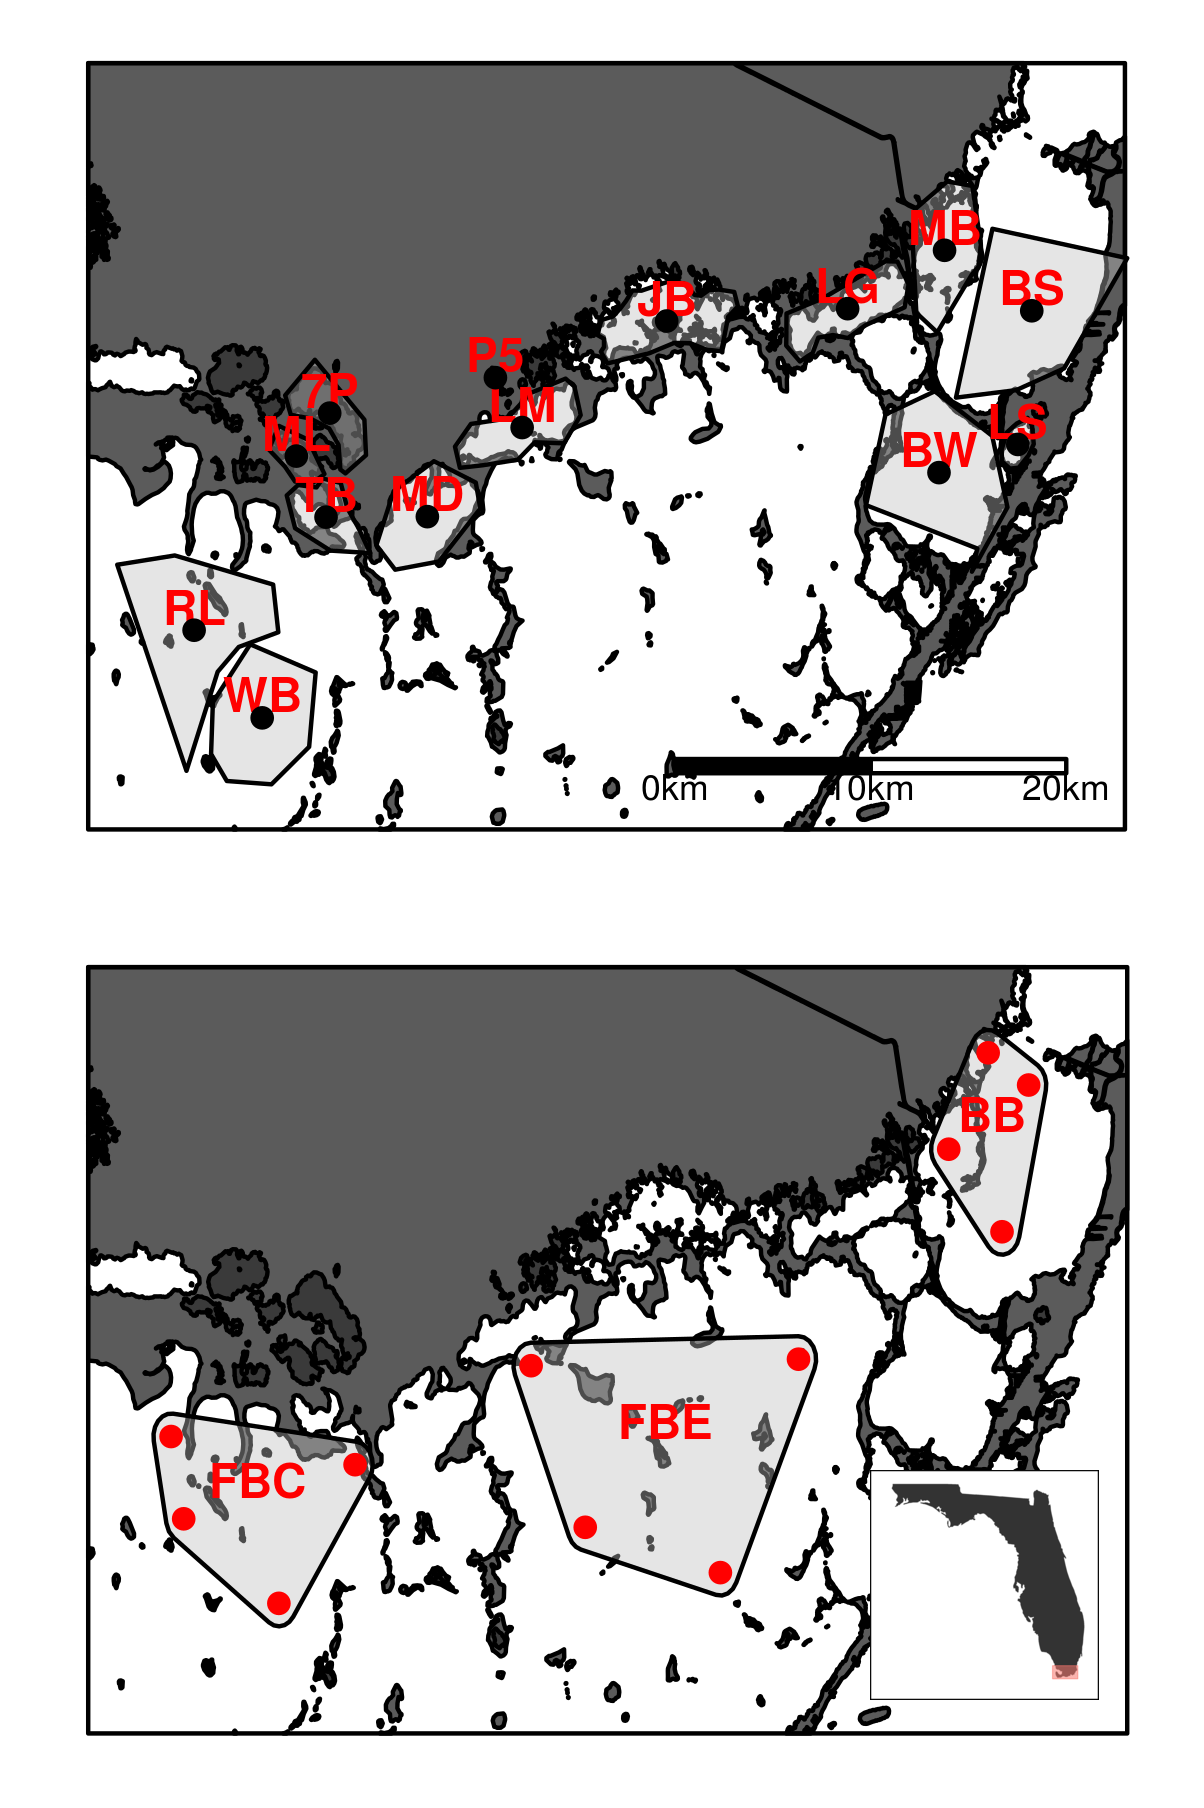
\includegraphics[width=0.75\textwidth]{../../figures/fbmap.png}
  \caption{Locations of discrete grab sampling sites within Florida Bay, USA. Polygons represent variability in sampling location over the course of the study period. a) Underway grab sampling network (1993-2015): RL = Rankin Lake, WB = Whipray Basin, TB = Terrapin Bay, ML = Monroe Lake, 7P = Seven Palm Lake, MD = Madeira Bay, LM = Little Madeira Bay, P5 = Pond Five, JB = Joe Bay, LG = Long Sound, BW = Blackwater Sound, LS = Lake Surprise, MB = Manatee Bay, BS = Barnes Sound; b) Long-term grab sampling network (2008-2015): BB – Biscayne Bay, FBE – Florida Bay East, FBC = Florida Bay Central.}
  \label{fig:1}
\end{figure*}

\newpage

\begin{figure*}
  \centering
  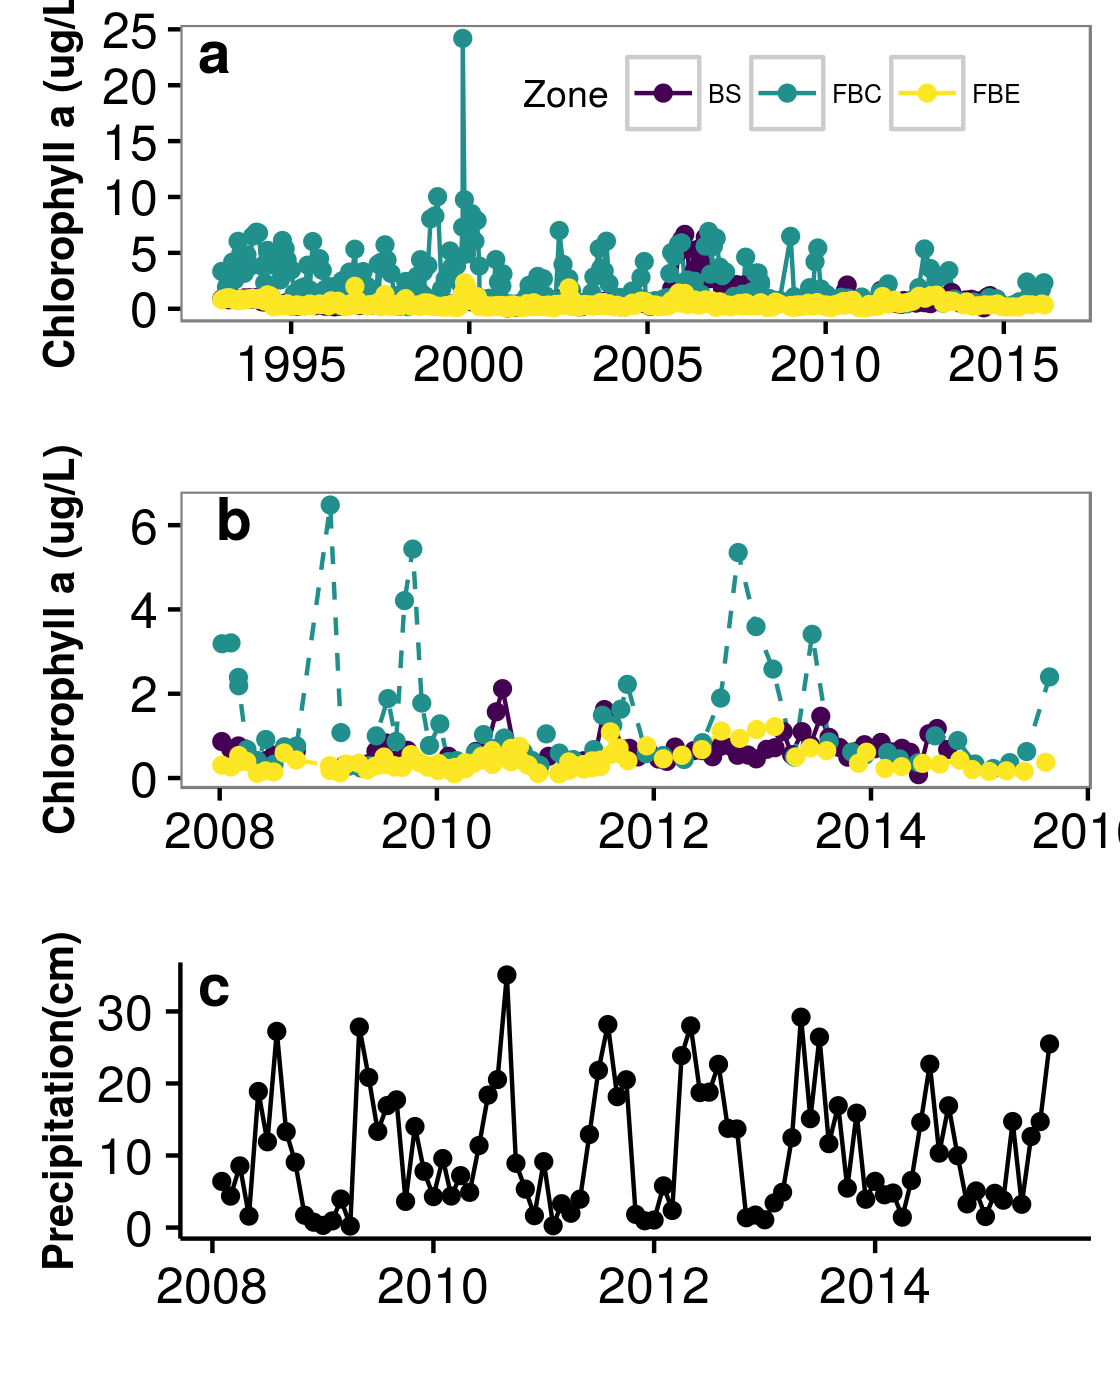
\includegraphics[width=0.75\textwidth]{../../figures/chltimeseries.png}
  \caption{a, b) Time series of average chlorophyll concentration within Florida Bay water quality zones. BS = Barnes Sound, FBC = Florida Bay Central, FBE = Florida Bay East. c) Precipitation during the study period. Precipitation data shown are cumulative monthly totals composited from three gages in the Florida Bay watershed.}
  \label{fig:2}
\end{figure*}

\newpage

\begin{figure*}
  \centering
  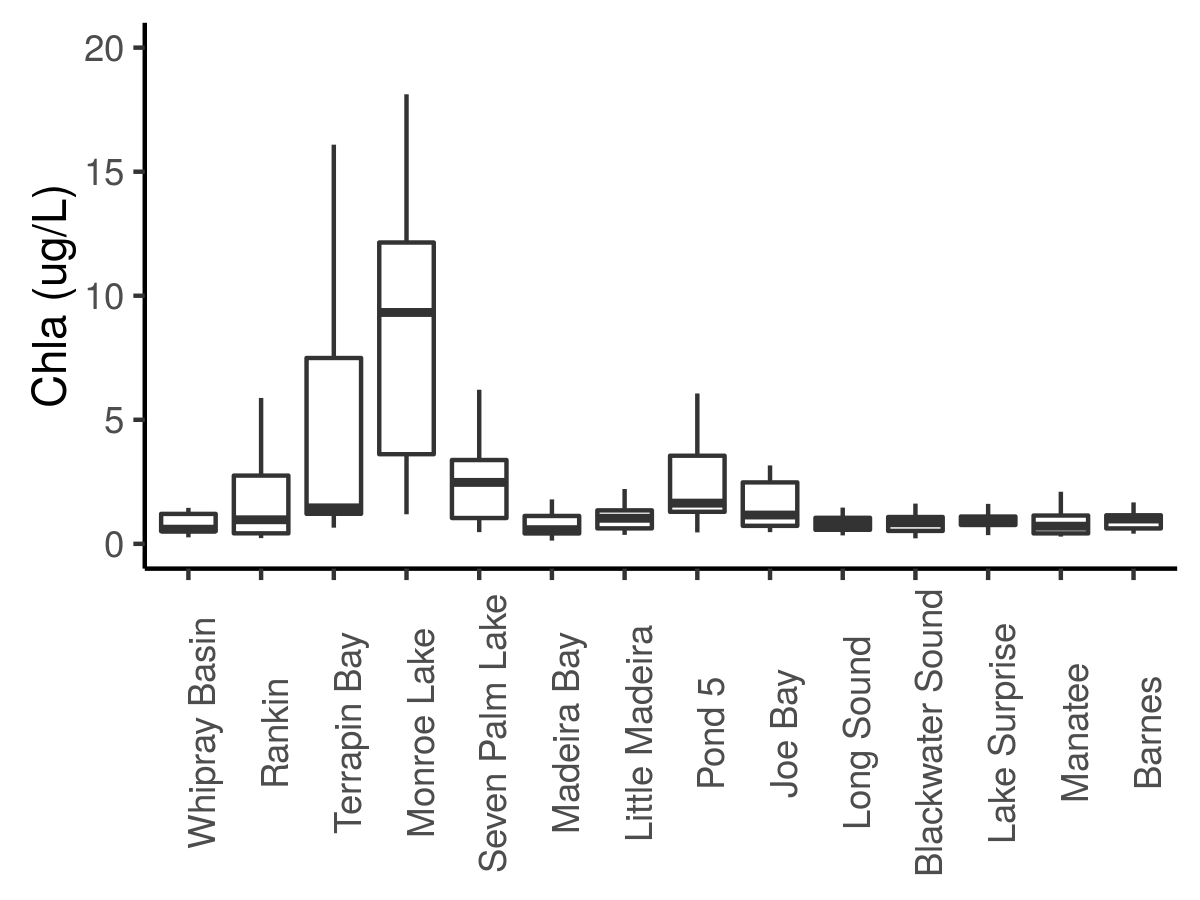
\includegraphics[width=0.75\textwidth]{../../figures/chlboxplot.png}
  \caption{Spatial distribution of chlorophyll concentration in selected Florida Bay basins. Basins are arranged geographically from west to east. The center line of each box is the median of the data, the height of the box represents the interquartile range, and the whiskers represent the fifth and 95th percentiles. }
  \label{fig:3}
\end{figure*}

\clearpage

\begin{figure*}
  \centering
  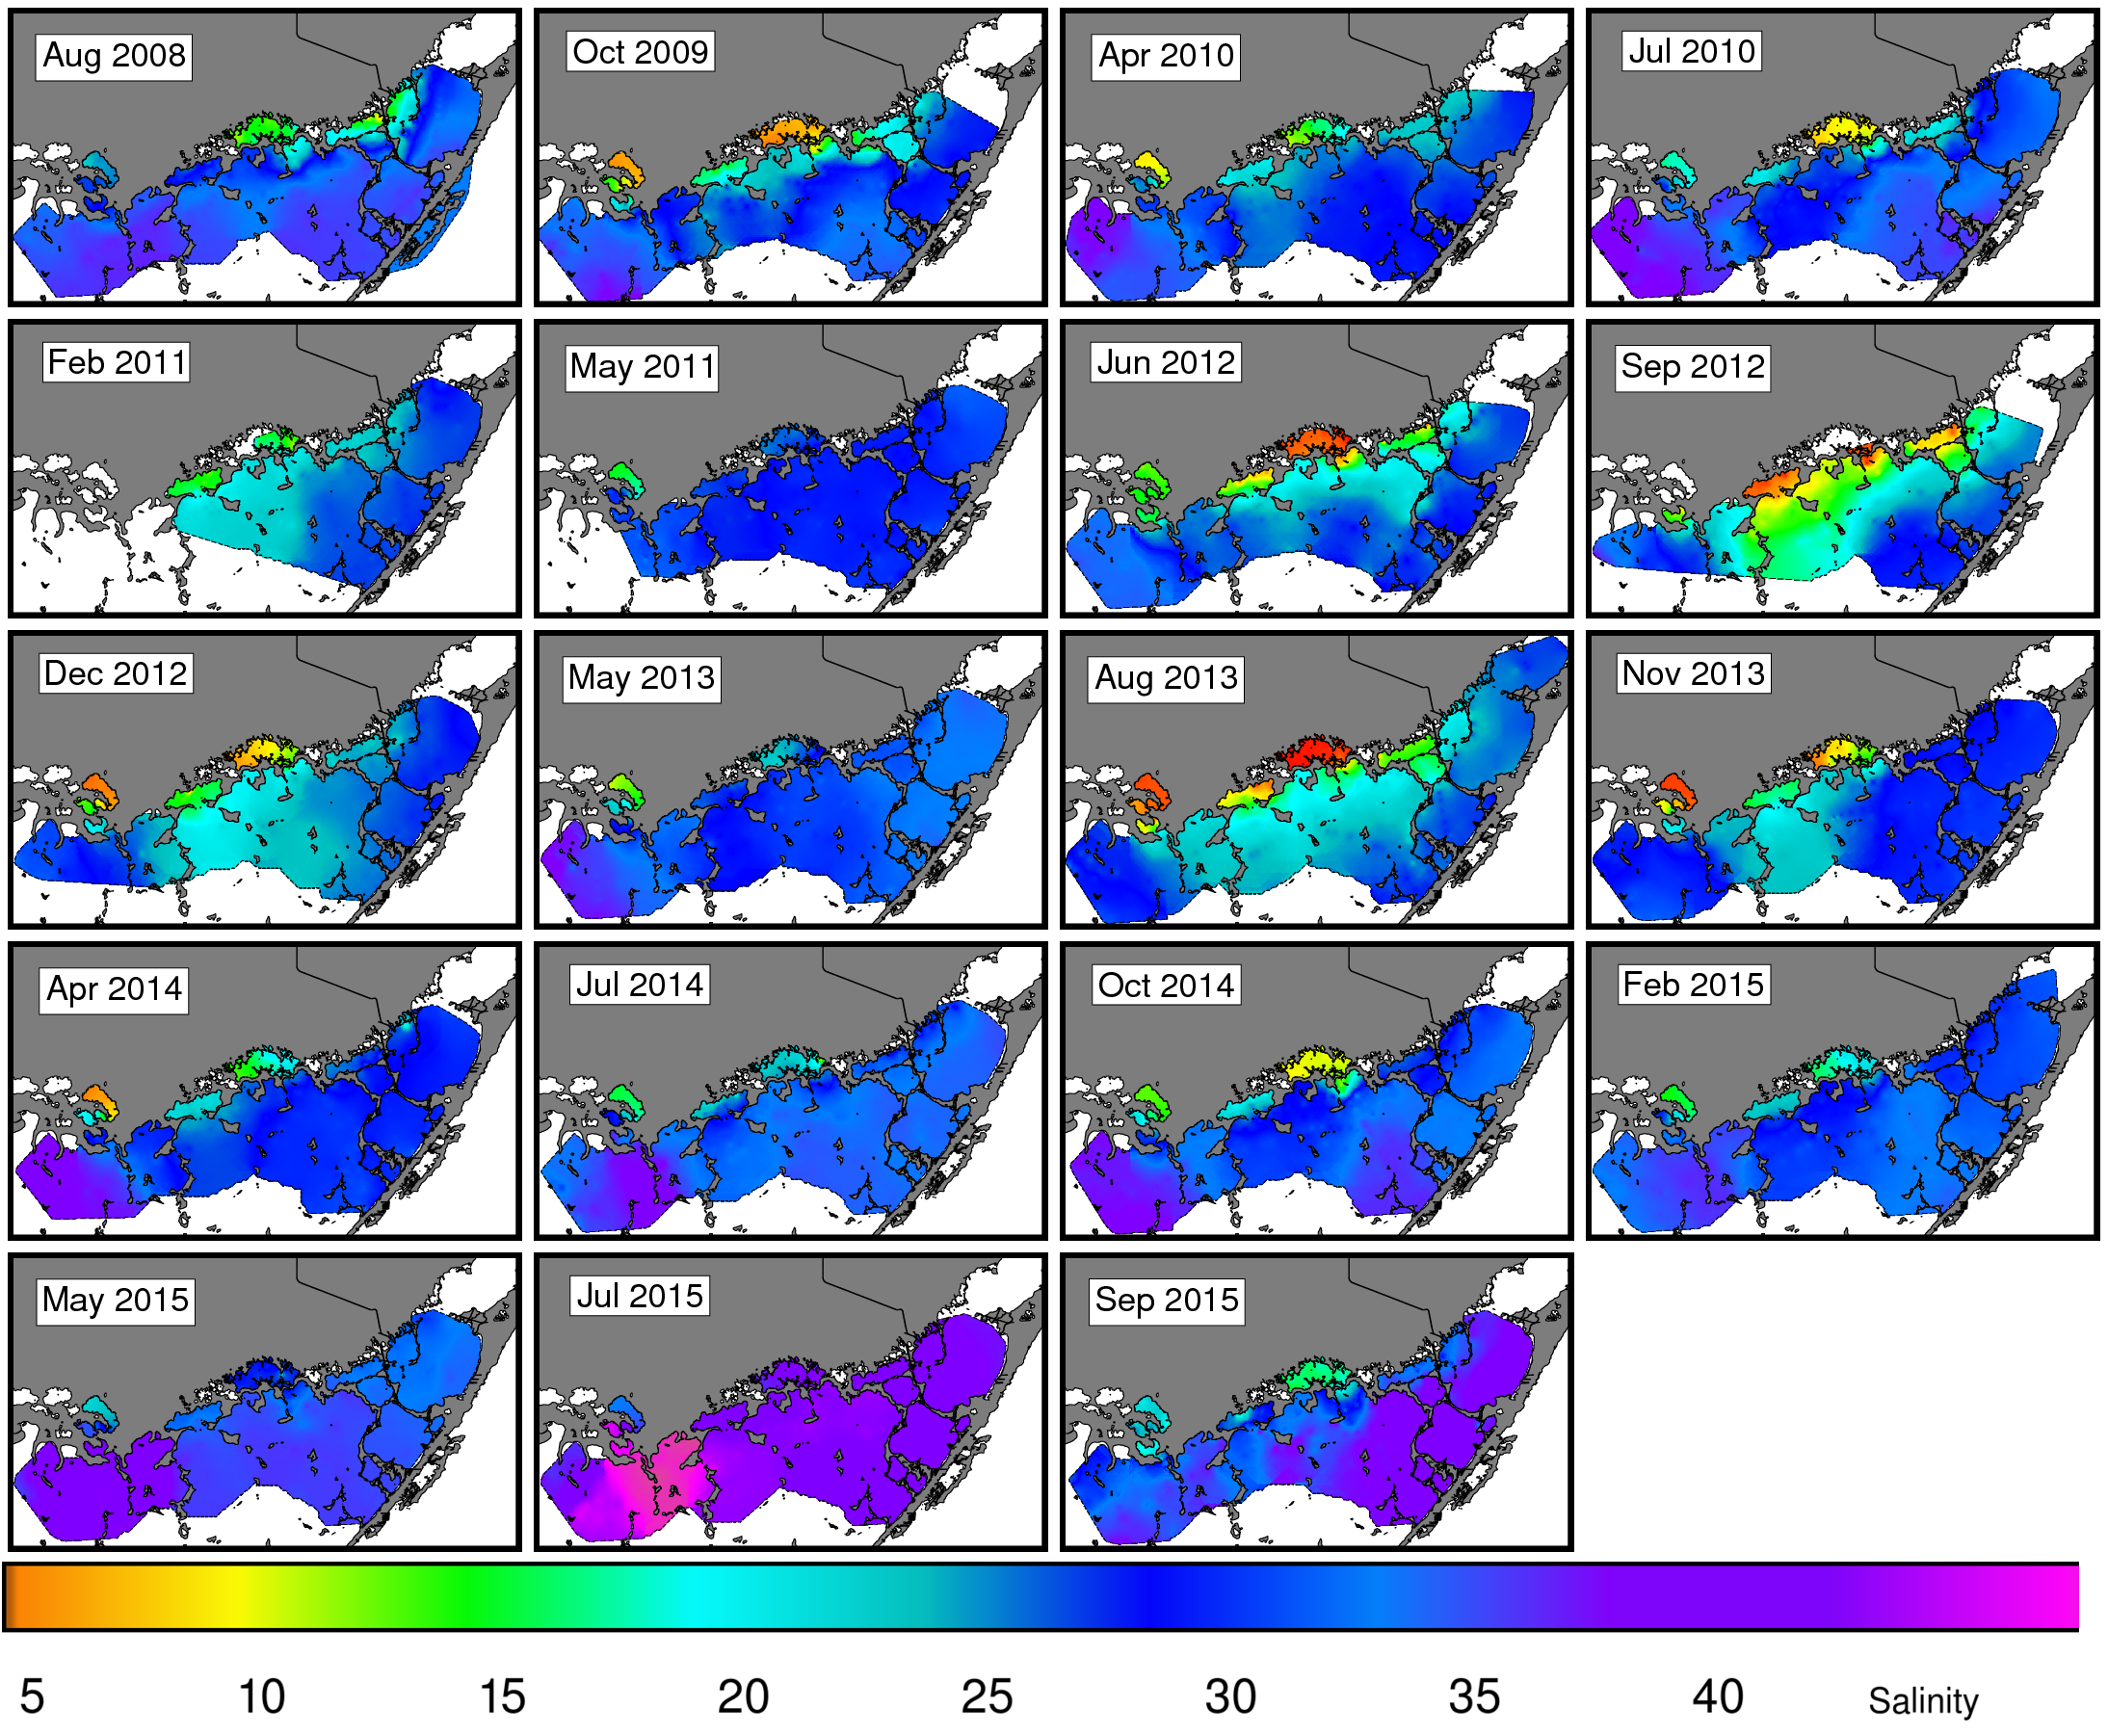
\includegraphics[width=0.9\textwidth]{../../figures/multipanel_salinity.png}
  \caption{Salinity surfaces for which a valid chlorophyll regression model could be developed. White areas denote areas that were not covered by underway surveys.}
  \label{fig:5}
\end{figure*}

\clearpage

\begin{figure*}
  \centering
  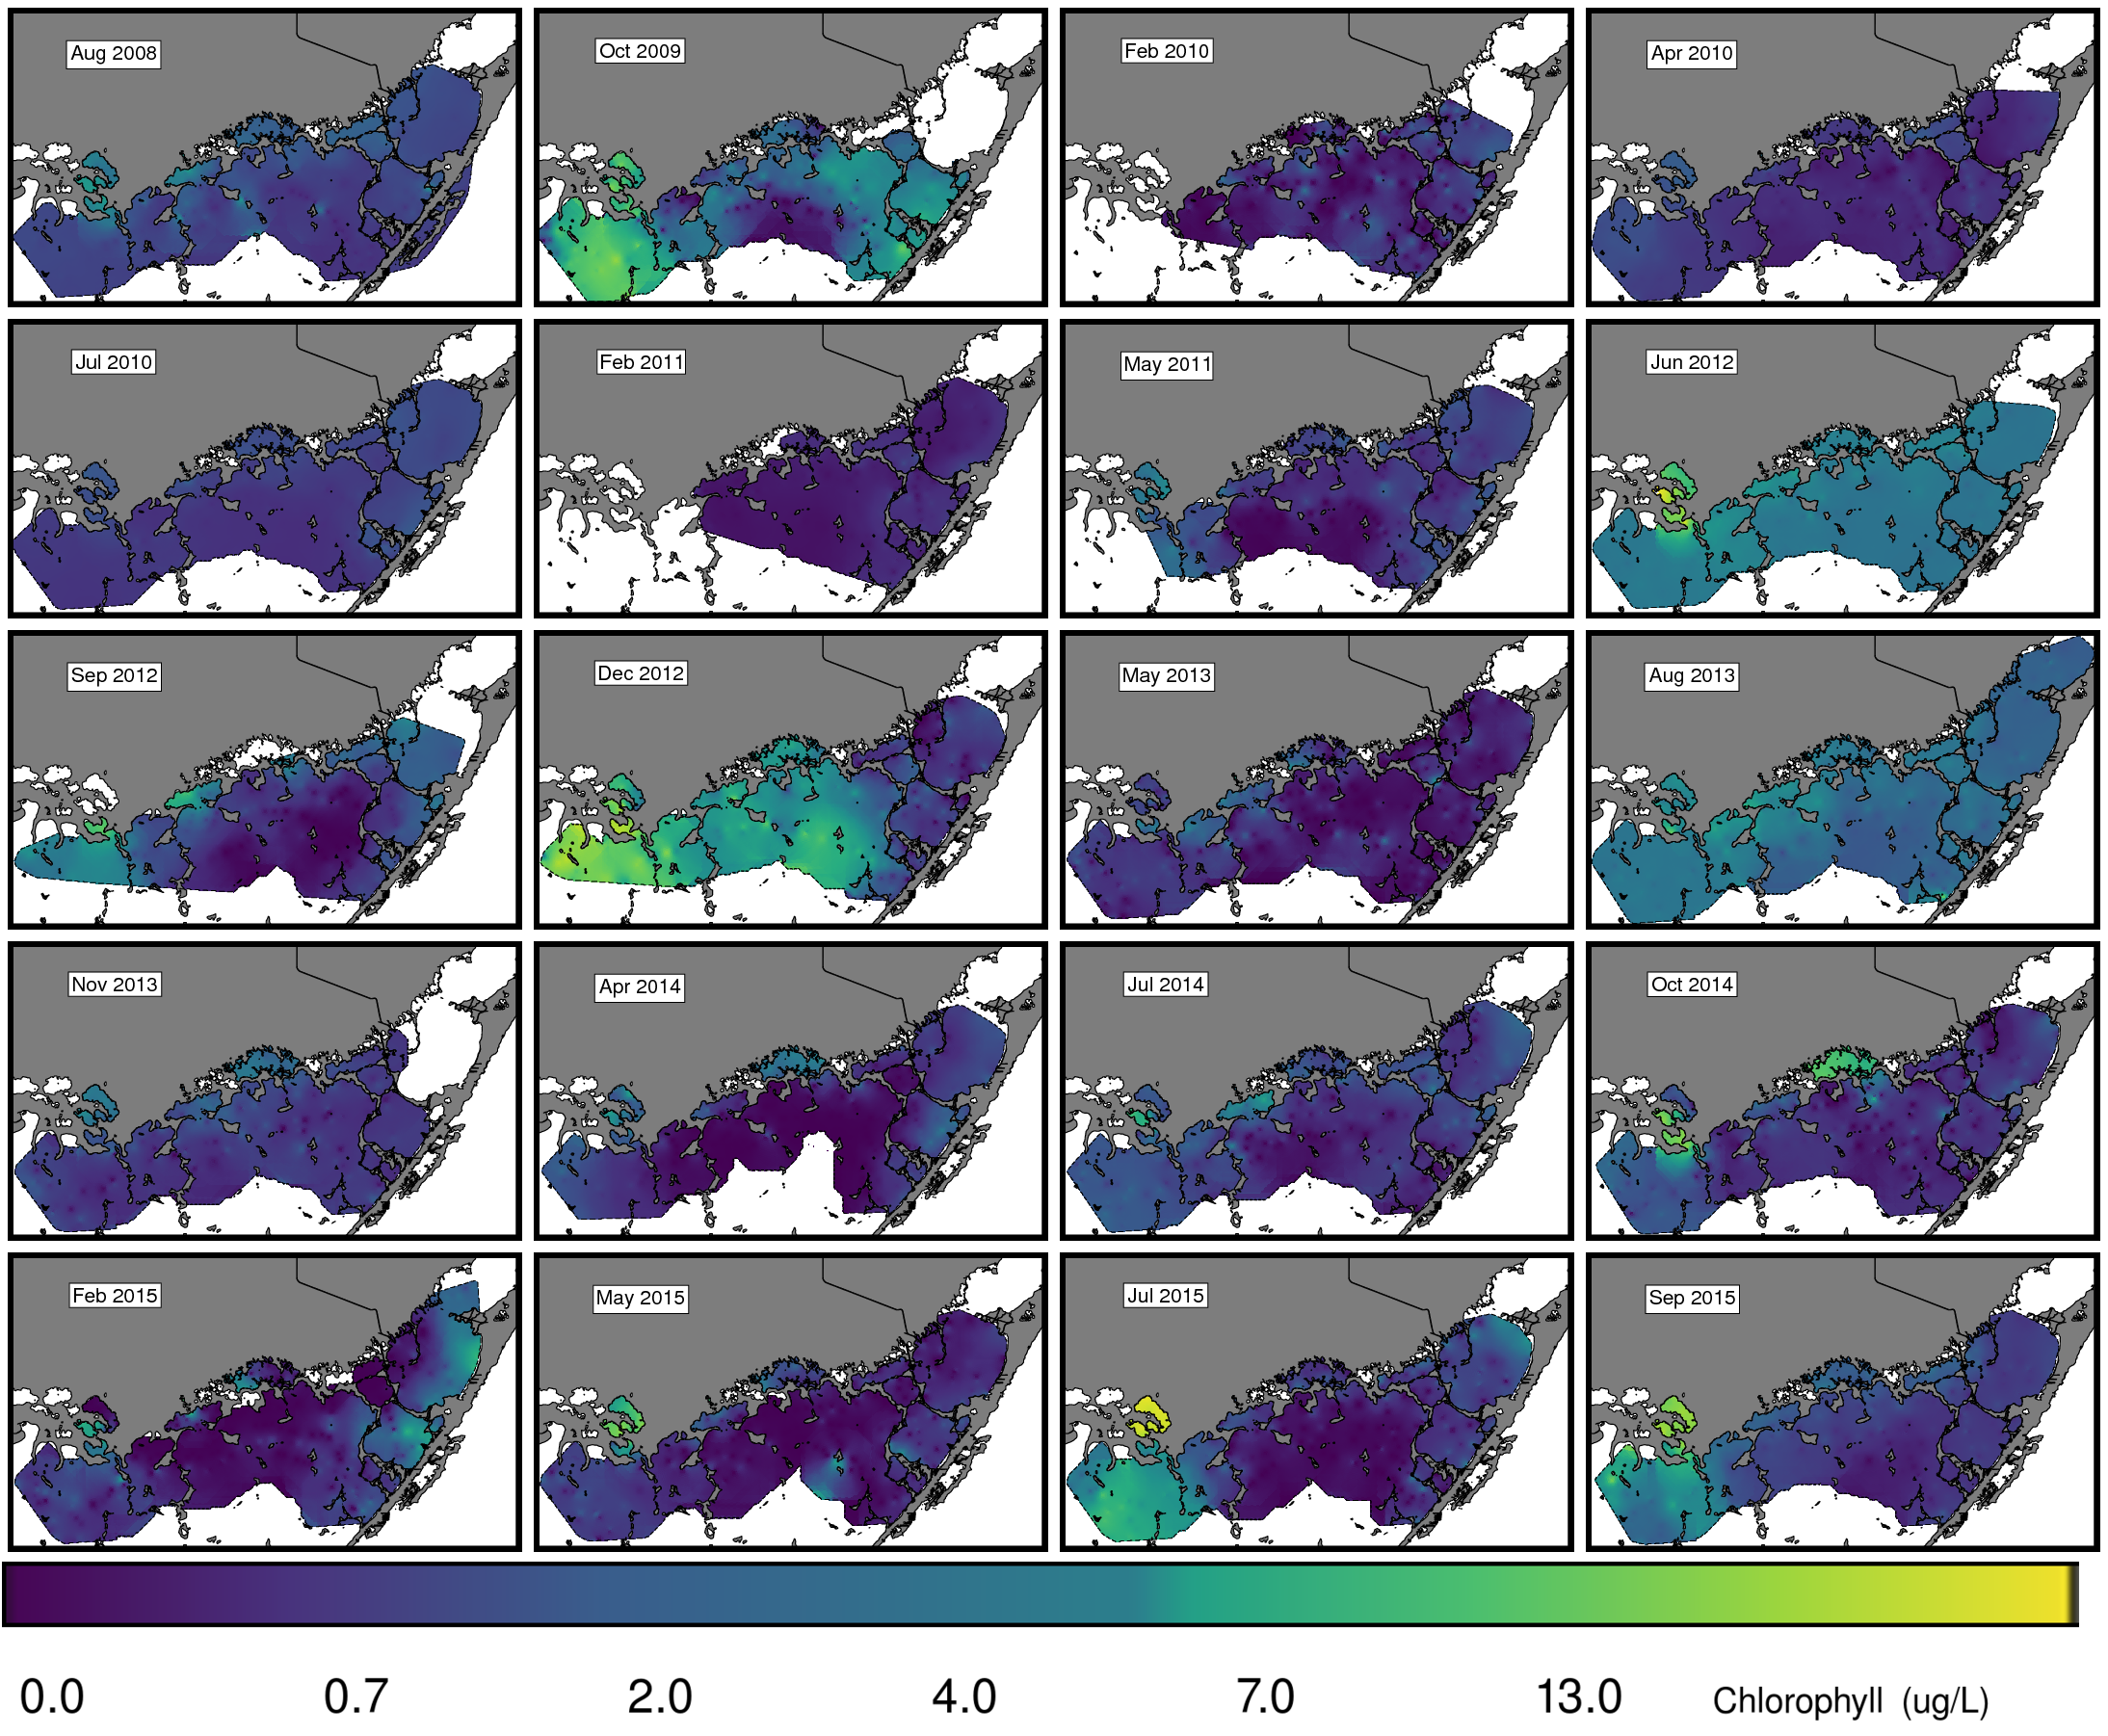
\includegraphics[width=0.9\textwidth]{../../figures/multipanel.png}
  \caption{Chlorophyll concentration surfaces calculated using the coefficients in Table 2. Surfaces shown are those for which a valid regression model could be developed. White areas denote areas that were not covered by underway surveys. Note that the color ramp is log-scaled.}
  \label{fig:4}
\end{figure*}

\clearpage

\begin{figure*}
  \centering
  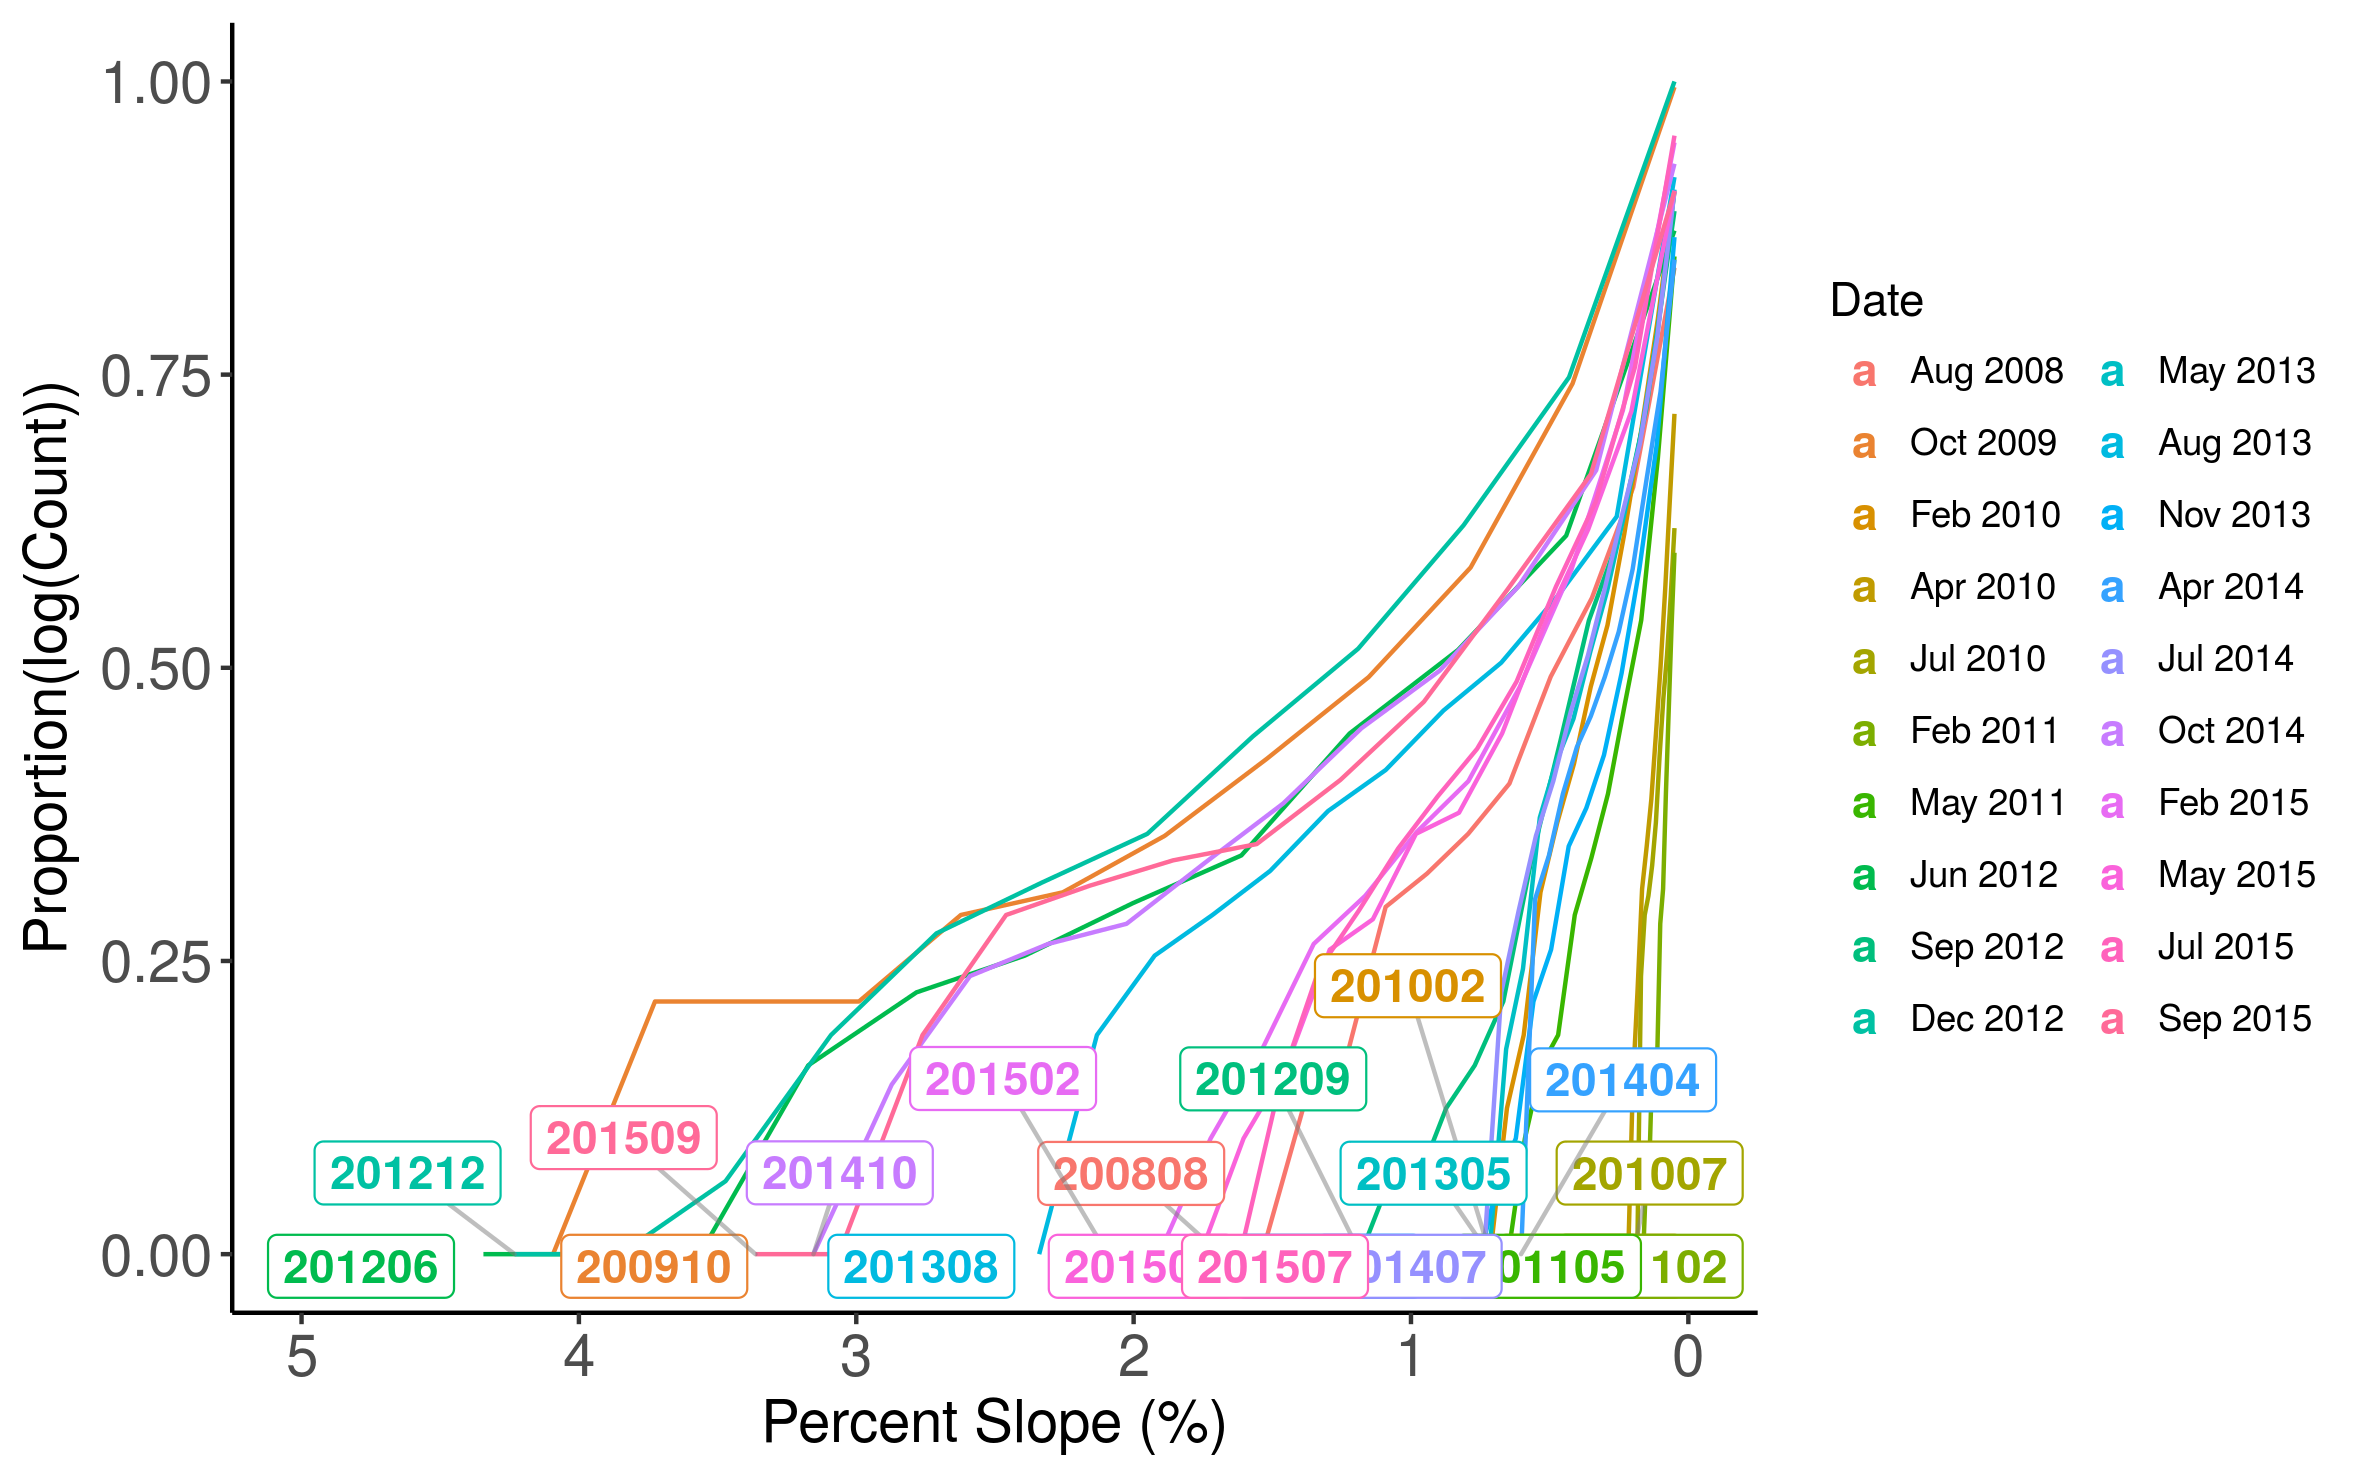
\includegraphics[width=0.85\textwidth]{../../figures/boundaries.png}
  \caption{Cumulative distribution of a) chlorophyll and b) salinity boundaries for each survey.}
  \label{fig:6}
\end{figure*}

\clearpage

% latex table generated in R 3.4.1 by xtable 1.8-2 package
% Tue Jul  4 16:26:09 2017
\begin{table}[ht]
\centering
\caption{Correlation matrix of water quality parameters for selected Florida Bay basins. TP = total phosphorus, TDP = total dissolved phosphorus, PO4 = ortho-phosphate, TN = total nitrogen, NH4 = ammonium, NO3 = nitrate, chla = chlorophyll a, PP = particulate phosphorus. $*$ indicates a significant correlation at P $<$ 0.05. Only complete cases were used in calculations (n = 86).} 
\begin{tabular}{rllllrll}
  \hline
 & TP & TDP & PO4 & TN & NH4 & NO3 & chla \\ 
  \hline
PP & 0.68* & 0.2 & 0.34* & 0.78* & 0.14 & -0.11 & 0.9* \\ 
  TP &  & 0.65* & 0.51* & 0.51* & 0.16 & 0.08 & 0.74* \\ 
  TDP &  &  & 0.48* & 0.09 & 0.18 & 0.3* & 0.28* \\ 
  PO4 &  &  &  & 0.36* & 0.16 & 0.19 & 0.4* \\ 
  TN &  &  &  &  & 0.17 & -0.12 & 0.67* \\ 
  NH4 &  &  &  &  &  & 0.55* & 0.19 \\ 
  NO3 &  &  &  &  &  &  & 0.02 \\ 
   \hline
\end{tabular}
\end{table}


\clearpage

\begin{figure*}
  \centering
  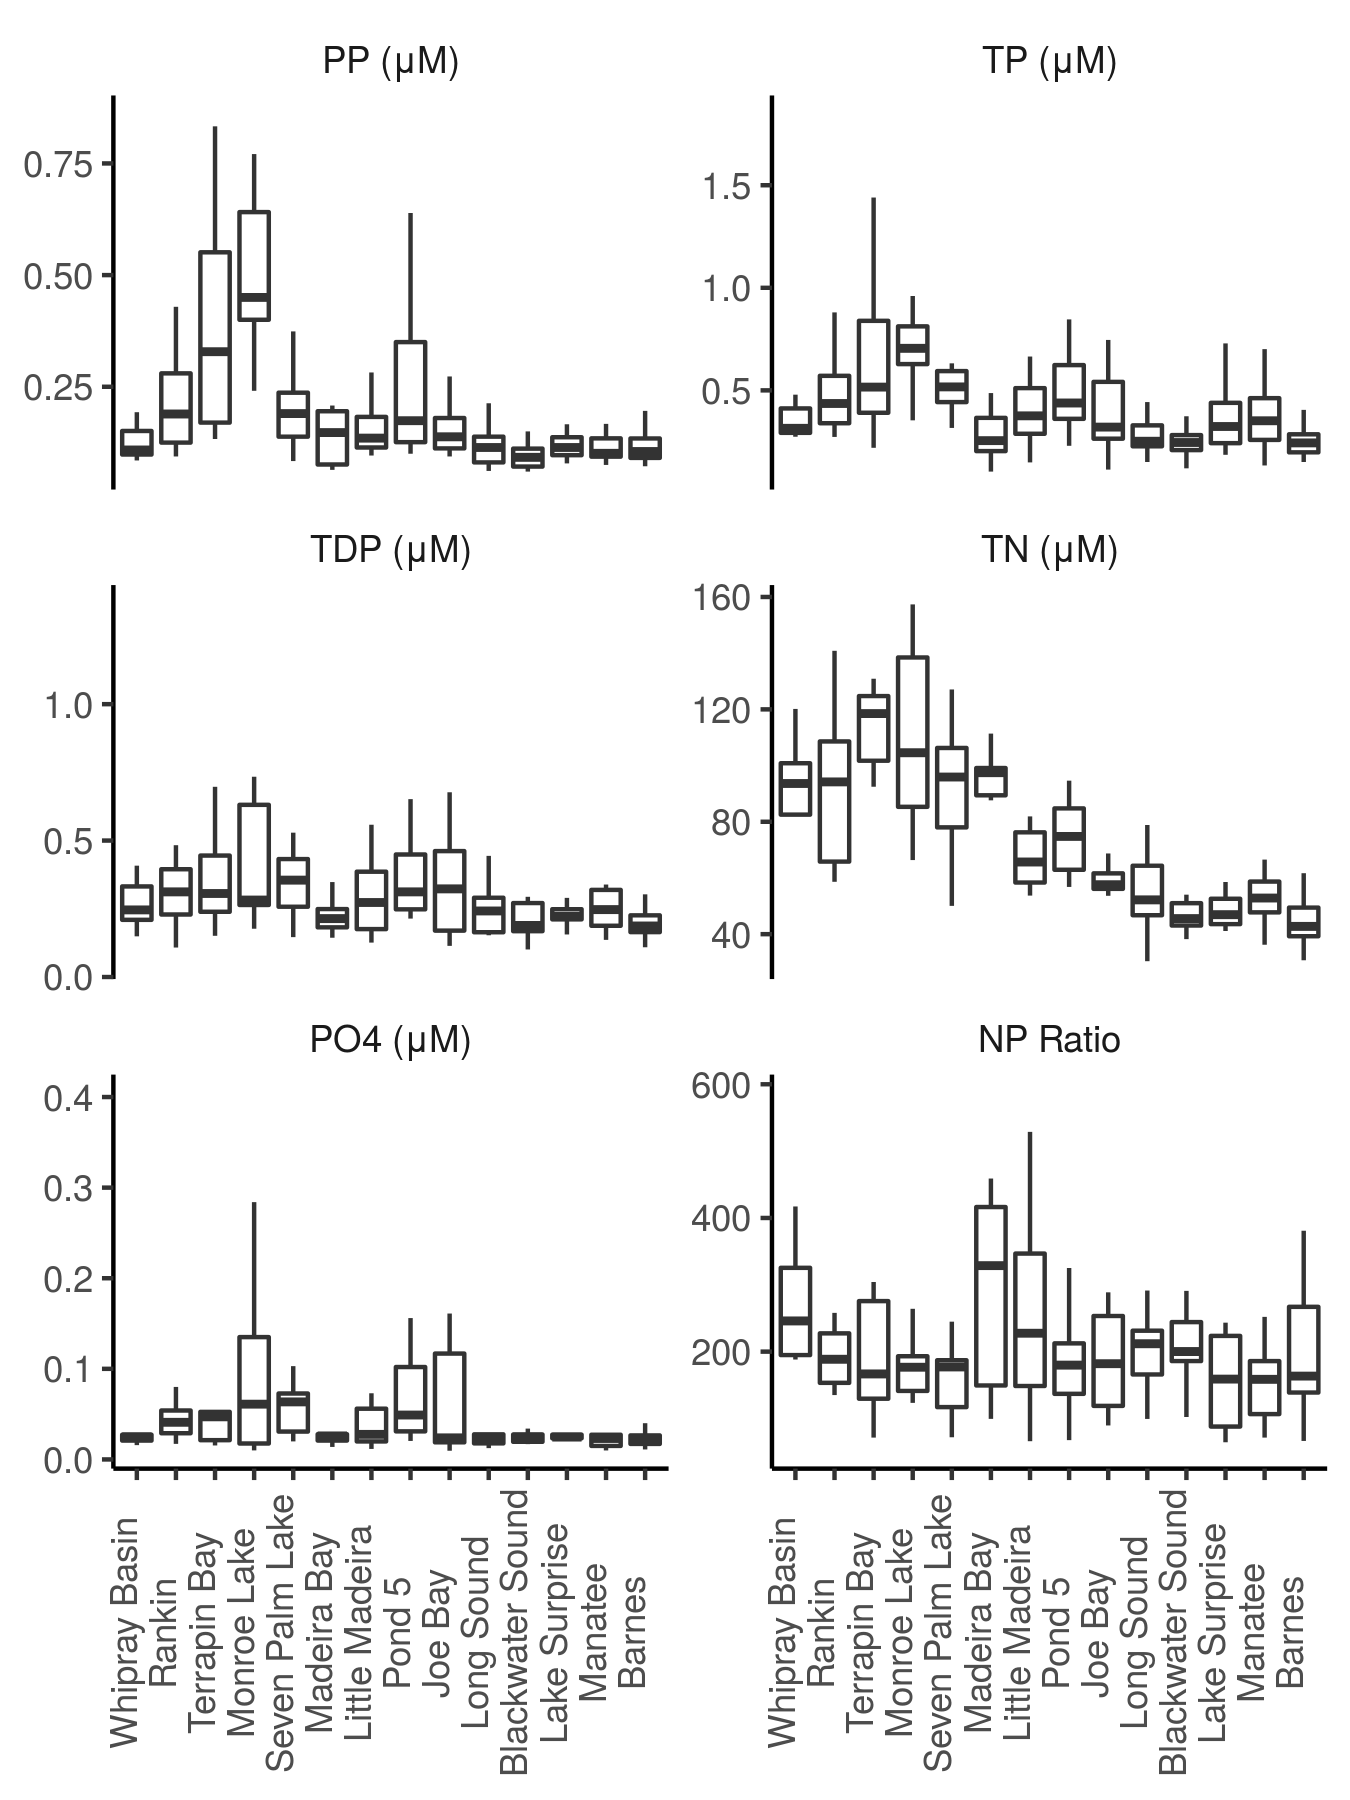
\includegraphics[width=0.75\textwidth]{../../figures/nonchlboxplot.png}
  \caption{Spatial distribution of discrete water quality parameters in selected Florida Bay basins.}
  \label{fig:7}
\end{figure*}

\newpage

\begin{table}

\caption{\label{tab:}Model coefficients for regressions between Dataflow and chlorophyll concentration of discrete grab samples. Also given is the coefficient of determination (R2) and p-value of each regression.}
\centering
\begin{tabular}[t]{lllllllllll}
\toprule
\multicolumn{1}{c}{ } & \multicolumn{2}{c}{Primary} & \multicolumn{4}{c}{Secondary} \\ \cmidrule(l{2pt}r{2pt}){2-3} \cmidrule(l{2pt}r{2pt}){4-7}
Date & CDOM & chla & PE & chla & CDOM & PC & intercept & $R^2$ & p & n\\
\midrule
2008-04 &  & 27.6258 &  &  &  &  & -4.6263 & 0.37 & 0.2 & 6\\
2008-08 &  & 5.1186 &  &  &  &  & -0.1353 & 0.9 & \textless0.01 & 10\\
2008-12 &  &  &  &  &  & 0.0509 & 0.0266 & 0.39 & 0.19 & 6\\
2009-10 & -67.1472 &  &  & 0.0495 &  &  & 6.2727 & 0.97 & \textless0.01 & 11\\
2010-02 &  &  & 0.0015 & 0.0025 & -2e-04 &  & -0.1338 & 0.63 & 0.5 & 10\\
\addlinespace
2010-04 &  & 7.8275 &  &  &  &  & -0.9164 & 0.69 & \textless0.01 & 14\\
2010-07 &  & 3.5643 &  &  &  &  & 0.0488 & 0.45 & 0.02 & 13\\
2011-02 &  &  &  & 0.0147 & -0.0011 &  & 0.0012 & 0.98 & \textless0.01 & 9\\
2011-05 &  & 12.5233 &  &  &  & 0.1473 & -3.1344 & 0.9 & \textless0.01 & 11\\
2012-06 &  &  &  &  &  & 0.0592 & 0.2531 & 0.84 & \textless0.01 & 12\\
\addlinespace
2012-09 &  & 20.2916 &  &  &  &  & -3.4262 & 0.84 & \textless0.01 & 10\\
2012-12 &  &  &  &  & 3e-04 & 0.143 & -1.2135 & 0.97 & \textless0.01 & 11\\
2013-05 &  &  &  &  &  & 0.2594 & -2.7694 & 0.96 & \textless0.01 & 14\\
2013-08 &  &  &  &  &  & 0.158 & -0.2626 & 0.68 & \textless0.01 & 15\\
2013-11 &  &  &  &  &  & 0.1864 & -1.4612 & 0.93 & \textless0.01 & 14\\
\addlinespace
2014-04 &  &  &  & 0.0217 &  &  & -1.3616 & 0.97 & \textless0.01 & 14\\
2014-07 &  &  & 0.0048 & 0.0019 &  & 0.1469 & -2.6215 & 0.91 & \textless0.01 & 14\\
2014-10 &  &  & -0.0011 &  & -5e-04 & 0.258 & -2.1036 & 0.99 & \textless0.01 & 14\\
2015-02 &  &  &  & 0.0121 & -5e-04 & 0.0485 & -0.9664 & 0.94 & \textless0.01 & 15\\
2015-05 &  &  &  &  &  & 0.2731 & -3.0247 & 0.74 & \textless0.01 & 14\\
\addlinespace
2015-07 &  &  &  &  &  & 0.3283 & -3.4682 & 0.97 & \textless0.01 & 14\\
2015-09 &  &  &  &  &  & 0.1184 & -0.8047 & 0.68 & \textless0.01 & 14\\
\bottomrule
\end{tabular}
\end{table}


\begin{figure*}
  \centering
  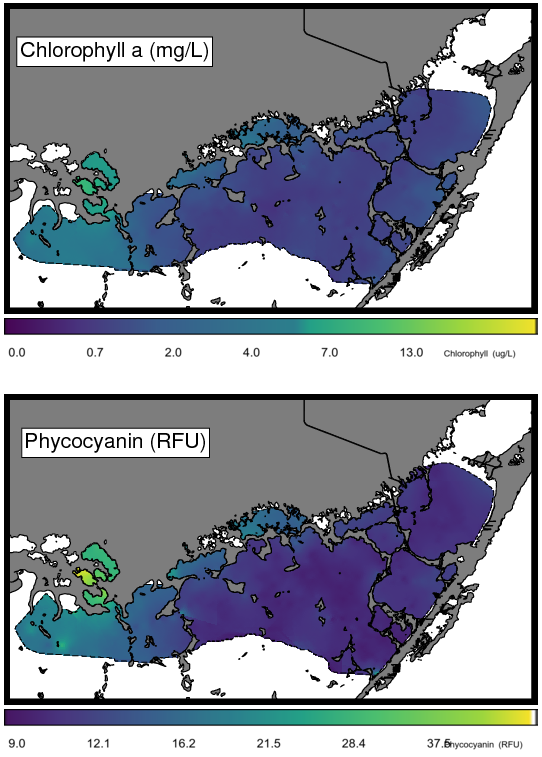
\includegraphics[width=0.65\textwidth]{../../figures/avmap.png}
  \caption{Maps of average chlorophyll a concentration and phycocyanin fluorescence.}
  \label{fig:7}
\end{figure*}

\end{document}
% end of file template.tex

